% ============================================================
%  Chapter 10 --- Constraints
%  Algorithms for Optimization, 2nd ed., Kochenderfer & Wheeler (2026)
%  Beamer slides  ---  aspectratio 16:9, Madrid/Seahorse theme
%  Reader-friendly version: complete sentences, symbol explanations,
%  worked examples, intuition-first exposition.
% ============================================================
\documentclass[aspectratio=169,10pt]{beamer}

\usetheme{Madrid}
\usecolortheme{seahorse}

% -- packages ----------------------------------------------
\usepackage[utf8]{inputenc}
\usepackage[T1]{fontenc}
\usepackage{amsmath,amssymb,amsfonts}
\usepackage{mathtools}
\usepackage{bm}
\usepackage{graphicx}
\usepackage{listings}
\usepackage{xcolor}
\usepackage{booktabs}
\usepackage{array}
\usepackage{tikz}
\usepackage{hyperref}

\graphicspath{{figures/}}

% -- listings style ----------------------------------------
\lstdefinestyle{pycode}{
  language=Python,
  basicstyle=\ttfamily\scriptsize,
  numbers=left,
  numberstyle=\tiny\color{gray},
  stepnumber=1,
  frame=single,
  backgroundcolor=\color{gray!7},
  keywordstyle=\color{blue!70!black}\bfseries,
  commentstyle=\color{green!50!black}\itshape,
  stringstyle=\color{red!70!black},
  breaklines=true,
  showstringspaces=false,
  tabsize=4,
  captionpos=b,
}

% -- footline ----------------------------------------------
\setbeamertemplate{footline}[frame number]

% -- macros ------------------------------------------------
\newcommand{\R}{\mathbb{R}}
\newcommand{\bx}{\mathbf{x}}
\newcommand{\bA}{\mathbf{A}}
\newcommand{\bb}{\mathbf{b}}
\newcommand{\bQ}{\mathbf{Q}}
\newcommand{\bL}{\mathbf{L}}
\newcommand{\by}{\mathbf{y}}
\newcommand{\blambda}{\bm{\lambda}}
\newcommand{\bmu}{\bm{\mu}}
\newcommand{\Lagr}{\mathcal{L}}
\DeclareMathOperator*{\minimize}{minimize}

% -- title info --------------------------------------------
\title[Ch.10 Constraints]{\textbf{Chapter 10: Constraints}}
\subtitle{Algorithms for Optimization, 2\textsuperscript{nd} Ed.\\
          Kochenderfer \& Wheeler (2026)}
\author{Lecture Slides}
\date{}

% ============================================================
\begin{document}
% ============================================================

% -- Title slide --------------------------------------------------------------
\begin{frame}
  \titlepage
\end{frame}

% -- Table of contents --------------------------------------------------------
\begin{frame}{Chapter Outline}
  \tableofcontents
\end{frame}

% =============================================================================
\section{Constrained Optimization}
% =============================================================================

\begin{frame}[allowframebreaks]{Why Constraints Arise}

  All of the optimization methods studied in previous chapters assume that the
  decision variable $\bx$ can take \emph{any} value in $\R^n$ (the set of all
  real $n$-dimensional vectors).  In practice, however, the physical or
  economic reality of a problem almost always restricts $\bx$ to a smaller set
  of \textbf{feasible} values.

  \begin{exampleblock}{Real-world examples where constraints are unavoidable}
    \begin{itemize}
      \item \textbf{Structural mechanics.}  The stress $\sigma$ (sigma) inside
            an aircraft wing cannot exceed a material limit
            $\sigma_{\max}$ (sigma sub max), otherwise the wing fails.
            This gives the inequality constraint $\sigma \le \sigma_{\max}$.

      \item \textbf{Portfolio allocation.}  If $w_i$ is the fraction of money
            invested in asset $i$, then the fractions must sum to exactly one
            (a budget equality constraint): $\sum_{i=1}^n w_i = 1$.  Here
            $\sum$ (Sigma) denotes the sum over all assets $i = 1, \ldots, n$.

      \item \textbf{Robot kinematics.}  Each joint has physical hard stops, so
            the joint angle $\theta$ (theta) is bounded:
            $\theta_{\min} \le \theta \le \theta_{\max}$.
    \end{itemize}
  \end{exampleblock}

  The set of all $\bx$ values that satisfy the constraints is called the
  \textbf{feasible set} $\mathcal{X}$.  When $\mathcal{X} \subsetneq \R^n$
  (strictly smaller than the full space), the problem is
  \textbf{constrained}.

  \framebreak

  \begin{columns}
    \begin{column}{0.52\textwidth}
      Adding a constraint does one of two things:

      \begin{enumerate}
        \item \textbf{It changes the optimum.}  The unconstrained minimum falls
              outside the feasible set, so we are forced to accept a worse (but
              feasible) solution at the boundary of $\mathcal{X}$.

        \item \textbf{It leaves the optimum unchanged.}  The unconstrained
              minimum already satisfies all constraints, so imposing them has no
              effect.
      \end{enumerate}

      The right-hand figure illustrates both cases.  The contours (level curves)
      of the objective $f$ are shown, together with a constraint boundary (a
      line).  In the middle panel the unconstrained minimum lies inside the
      feasible region, so the constraint is \emph{inactive}.  In the right panel
      the minimum lies outside, so the constraint is \emph{active} and the
      solution moves to the boundary.

    \end{column}
    \begin{column}{0.46\textwidth}
      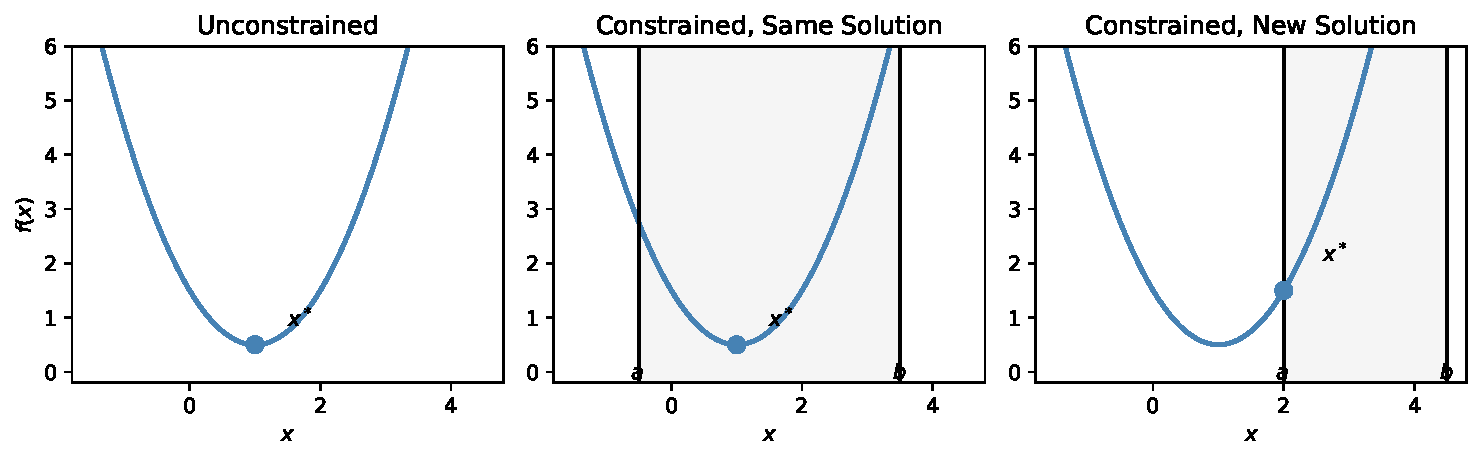
\includegraphics[width=\linewidth]{constraint_effect.pdf}
      \begin{center}
        \scriptsize A constraint can shift the optimum to the boundary (right
        panel) or leave it unchanged when it is already feasible (middle panel).
      \end{center}
    \end{column}
  \end{columns}

  \begin{alertblock}{Key Insight}
    Whether a constraint ``matters'' depends entirely on where the unconstrained
    minimum sits relative to the feasible set.  A core goal of this chapter is
    to develop methods that efficiently find the constrained optimum regardless
    of which case applies.
  \end{alertblock}

\end{frame}

% -----------------------------------------------------------------------------

\begin{frame}[allowframebreaks]{The General Constrained Optimization Problem}

  The most common way to write a constrained optimization problem unifies all
  constraint types into a single \emph{standard form}.

  \begin{block}{Standard Form (Eq.~10.2)}
    \[
      \minimize_{\bx}\; f(\bx) \qquad
      \begin{array}{ll}
        \text{subject to} & h_i(\bx) = 0, \quad i = 1,\ldots,\ell \\
                          & g_j(\bx) \le 0, \quad j = 1,\ldots,m
      \end{array}
    \]
  \end{block}

  \begin{block}{Notation}
    \begin{itemize}
      \item $\bx \in \R^n$ (x bold) is the \textbf{design vector} --- the $n$
            variables we are optimizing over.
      \item $f : \R^n \to \R$ is the \textbf{objective function} --- the scalar
            quantity we want to minimize.
      \item $h_i : \R^n \to \R$ (h sub i) are the $\ell$ (ell)
            \textbf{equality constraints}.  Requiring $h_i(\bx)=0$ pins $\bx$
            to a surface of dimension $n-\ell$.
      \item $g_j : \R^n \to \R$ (g sub j) are the $m$
            \textbf{inequality constraints}.  The convention $g_j(\bx)\le 0$
            means the constraint is satisfied when the function value is zero or
            negative.
    \end{itemize}
  \end{block}

  \framebreak

  \begin{alertblock}{How to Read This Formula}
    Reading the standard form aloud: ``minimize $f(\bx)$ over all choices of
    $\bx$, subject to the requirement that each equality function $h_i$ equals
    zero, and each inequality function $g_j$ is at most zero.''  The word
    \emph{subject to} (often abbreviated \emph{s.t.}) means ``while also
    satisfying''.
  \end{alertblock}

  \medskip
  \textbf{Converting other forms.}  At first glance it may seem that only
  $\le$ inequalities are handled.  In fact, any constraint can be rewritten in
  this form:

  \begin{itemize}
    \item A greater-than constraint $g(\bx) \ge 0$ is equivalent to $-g(\bx) \le 0$,
          so simply negate the function.
    \item A strict equality $h(\bx) = 0$ is already in the form above.
    \item A set-membership requirement $\bx \in \mathcal{X}$ (for some
          geometric set $\mathcal{X}$) can often be converted to a collection
          of inequality functions.
  \end{itemize}

  \begin{exampleblock}{Worked Example --- writing a problem in standard form}
    Suppose we want to minimize $x_1^2 + x_2^2$ (the squared distance from the
    origin) subject to: the point lying on the line $x_1 + x_2 = 1$, and both
    coordinates being non-negative.

    \medskip
    In standard form:
    \begin{align*}
      \minimize_{x_1, x_2}\; & x_1^2 + x_2^2 \\
      \text{s.t.}\;           & h(x_1,x_2) = x_1 + x_2 - 1 = 0\quad\text{(equality)}\\
                              & g_1(x_1,x_2) = -x_1 \le 0\quad\text{(i.e.\ $x_1 \ge 0$)}\\
                              & g_2(x_1,x_2) = -x_2 \le 0\quad\text{(i.e.\ $x_2 \ge 0$)}
    \end{align*}
    Note that $x_i \ge 0$ becomes $-x_i \le 0$ by negation.
  \end{exampleblock}

\end{frame}

% =============================================================================
\section{Constraint Types}
% =============================================================================

\begin{frame}[allowframebreaks]{A Taxonomy of Constraint Types}

  While the standard form uses only equalities and $\le$ inequalities, it is
  helpful to recognise the different geometric shapes these constraints produce,
  because some algorithms exploit that geometry directly.

  \begin{block}{1. Equality Constraints --- $h(\bx) = 0$}
    An equality constraint restricts $\bx$ to a \textbf{surface} (technically a
    manifold) embedded in $\R^n$.  With $\ell$ independent equality constraints,
    the feasible surface has dimension $n - \ell$.  For instance, with $n = 3$
    variables and one equality constraint ($\ell = 1$), the feasible set is a
    two-dimensional surface inside three-dimensional space.
  \end{block}

  \begin{block}{2. Inequality Constraints --- $g(\bx) \le 0$}
    An inequality constraint restricts $\bx$ to one \textbf{side} of a surface:
    the set $\{\ \bx : g(\bx) \le 0\ \}$ is a closed half-space (if $g$ is
    linear) or a curved feasible region (if $g$ is nonlinear).  The boundary
    $g(\bx) = 0$ is called the \textbf{constraint boundary}.
  \end{block}

  \begin{block}{3. Bound and Box Constraints --- $a \le x_i \le b$}
    A bound constraint on the $i$-th component can be written as two inequality
    constraints:
    \[
      g_1(x_i) = x_i - b \le 0 \quad\text{and}\quad g_2(x_i) = a - x_i \le 0.
    \]
    When bounds are placed on \emph{every} component simultaneously,
    $\mathbf{a} \le \bx \le \mathbf{b}$, the feasible set is a
    \textbf{box} (a hyperrectangle in $\R^n$).
  \end{block}

  \framebreak

  The following table summarises all constraint types and their unified
  representations in standard form.

  \vspace{6pt}
  \begin{tabular}{lll}
    \toprule
    \textbf{Type}   & \textbf{Form}              & \textbf{Geometric meaning} \\
    \midrule
    Equality        & $h(\bx) = 0$               & Surface / manifold \\
    Inequality      & $g(\bx) \le 0$             & Half-space or curved region \\
    Bound           & $a \le x_i \le b$          & Interval on one axis \\
    Box             & $\bx \in [\mathbf{a}, \mathbf{b}]$ & Hyperrectangle \\
    Set-membership  & $\bx \in \mathcal{X}$      & Any closed set \\
    \bottomrule
  \end{tabular}

  \vspace{10pt}

  \begin{alertblock}{Key Insight}
    Because any constraint type can be converted to equality or inequality form,
    we only need to develop algorithms that handle these two types --- and those
    algorithms will apply universally to all constrained problems.
  \end{alertblock}

\end{frame}

% =============================================================================
\section{Transformations to Remove Constraints}
% =============================================================================

\begin{frame}[allowframebreaks]{Removing Bound Constraints via Variable Transformation}

  One of the most elegant strategies for handling a bound constraint
  $a \le x \le b$ is to \textbf{transform the variable} so that the bound is
  automatically satisfied.  We introduce an \emph{unconstrained} helper
  variable $\hat{x}$ (x-hat) that can take any real value, and define $x$ as
  a function $t_{a,b}(\hat{x})$ that always maps into $(a, b)$.  Because $x$
  can never violate the bound by construction, the constraint disappears from
  the problem statement entirely, and any unconstrained solver can be applied to
  the transformed problem.

  \begin{block}{The Sinusoidal Bound Transform}
    \[
      x = t_{a,b}(\hat{x}) = a + (b - a)\,\sin^2(\hat{x})
    \]
  \end{block}

  \begin{block}{Notation and How to Read This}
    \begin{itemize}
      \item $a$ and $b$ are the lower and upper bounds, respectively
            (e.g., $a = 2$, $b = 6$).
      \item $\hat{x}$ (x-hat) is the \textbf{unconstrained} helper variable;
            it can be any real number.
      \item $\sin^2(\hat{x})$ (sine squared of x-hat) always lies in $[0, 1]$
            regardless of the value of $\hat{x}$, because sine is always between
            $-1$ and $1$.
      \item Therefore $t_{a,b}(\hat{x})$ always lies in $[a, a + (b-a) \cdot 1]
            = [a, b]$, satisfying the bound automatically.
    \end{itemize}
    The formula maps an infinite real line onto the bounded interval $[a, b]$,
    wrapping back and forth like a sinusoid.  Every value inside $(a, b)$ is
    achieved by infinitely many values of $\hat{x}$.
  \end{block}

  \framebreak

  \textbf{Procedure.}  To minimize $f(x)$ subject to $a \le x \le b$:
  \begin{enumerate}
    \item Define the helper variable $\hat{x} \in \R$ (unconstrained).
    \item Substitute $x = t_{a,b}(\hat{x})$ into $f$ to get a new function
          $\tilde{f}(\hat{x}) = f\!\bigl(t_{a,b}(\hat{x})\bigr)$.
    \item Minimize $\tilde{f}$ over $\hat{x}$ using any unconstrained
          algorithm (gradient descent, L-BFGS, etc.).
    \item Convert the solution $\hat{x}^*$ back to $x^* = t_{a,b}(\hat{x}^*)$.
  \end{enumerate}

  \begin{columns}
    \begin{column}{0.55\textwidth}
      \begin{exampleblock}{Worked Example 10.1 --- $\min\; x\sin(x)$, $x \in [2, 6]$}
        The function $f(x) = x\sin(x)$ has several local minima on $[2, 6]$.
        After transformation, $\tilde{f}(\hat{x}) = t_{2,6}(\hat{x})\cdot\sin\!\bigl(t_{2,6}(\hat{x})\bigr)$
        is an unconstrained function on $\R$.

        \medskip
        Running L-BFGS from multiple starting points finds two minima in
        $\hat{x}$-space at approximately $\hat{x} \approx 0.242$ and
        $\hat{x} \approx 4.139$, both mapping back to
        $x^* \approx 4.914$ in the original space.

        \medskip
        The optimal value is $f^* \approx -4.814$.
      \end{exampleblock}
    \end{column}
    \begin{column}{0.43\textwidth}
      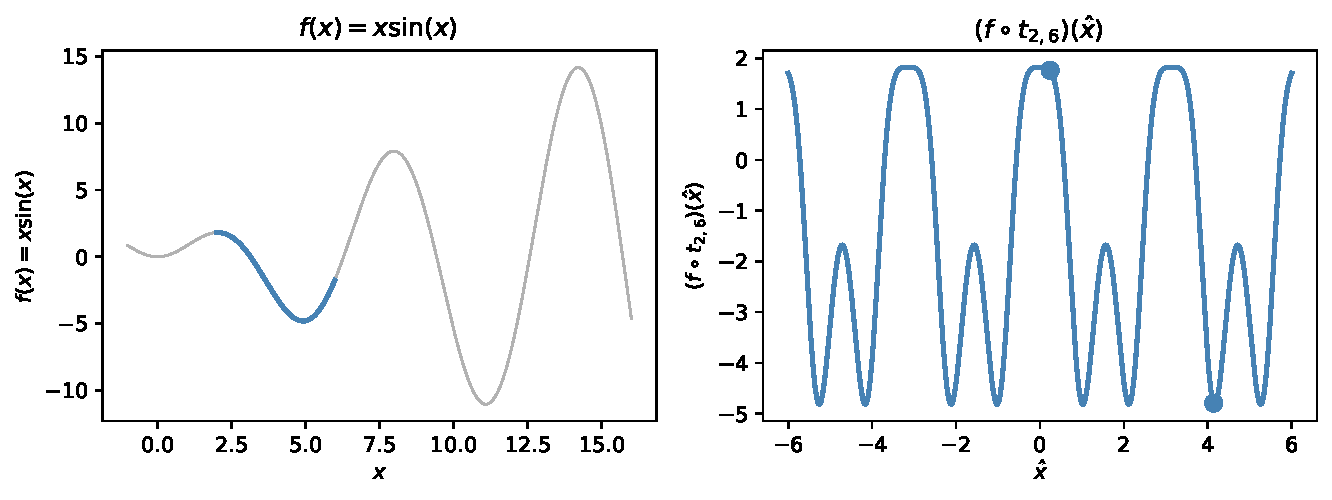
\includegraphics[width=\linewidth]{bound_transform_ex10_1.pdf}
      \begin{center}
        \scriptsize Top: original $f(x)$ on $[2,6]$.  Bottom:
        transformed $\tilde{f}(\hat{x})$ on $\R$.  Two local
        minima in $\hat{x}$ both correspond to the same $x^*$.
      \end{center}
    \end{column}
  \end{columns}

  \begin{alertblock}{Key Insight}
    The transformation trades a constrained problem for an unconstrained one,
    but it introduces \emph{multiple pre-images} (several $\hat{x}$ values
    correspond to the same $x$), which can create spurious local minima.
    Running from multiple starting points mitigates this.
  \end{alertblock}

\end{frame}

\begin{frame}[fragile]{Python: Bound-Constrained Minimization via Transform}
  \begin{lstlisting}[style=pycode,caption={Example 10.1 in Python --- bound-constrained minimization using sinusoidal transform}]
import numpy as np
from scipy.optimize import minimize

a, b = 2.0, 6.0

def t(xhat):
    """Sinusoidal transform: maps any real xhat into (a, b)."""
    return a + (b - a) * np.sin(xhat)**2

def f_transformed(xhat):
    x = t(xhat)
    return x * np.sin(x)

# Solve unconstrained problem from many starting points to avoid local minima
results = []
for x0 in np.linspace(-6, 6, 20):
    res = minimize(f_transformed, x0, method='L-BFGS-B')
    results.append((res.fun, t(res.x[0])))

# Best solution in original space
best = min(results, key=lambda r: r[0])
print(f"f* = {best[0]:.4f},  x* = {best[1]:.4f}")
# Output: f* = -4.8141,  x* = 4.9136
  \end{lstlisting}
\end{frame}

% =============================================================================
\section{Removing Affine Equality Constraints}
% =============================================================================

\begin{frame}[allowframebreaks]{Removing Affine Equality Constraints via LQ Decomposition}

  An \textbf{affine equality constraint} has the form $\bA\bx = \bb$, where
  $\bA \in \R^{m \times n}$ is a matrix of coefficients and $\bb \in \R^m$ is
  a constant vector.  For example, ``the sum of all portfolio weights equals
  one'' is an affine constraint.

  The idea is to perform a change of variables that \textbf{automatically
  satisfies} the equality, so the constraint can be dropped entirely.  We do
  this using the \textbf{LQ decomposition} of $\bA$.

  \begin{block}{LQ Decomposition of $\bA$ (Eq.~10.6)}
    \[
      \bA = \begin{bmatrix}\bL & \mathbf{0}\end{bmatrix}\bQ
    \]
  \end{block}

  \begin{block}{Notation}
    \begin{itemize}
      \item $\bA \in \R^{m \times n}$ (A bold) is the constraint coefficient
            matrix, with $m$ rows (one per equality constraint) and $n$ columns
            (one per variable).  We assume $m < n$ (fewer constraints than
            variables) and that $\bA$ has full row rank $m$.
      \item $\bL \in \R^{m \times m}$ (L bold) is a \textbf{lower-triangular}
            matrix --- meaning all entries above the main diagonal are zero.
            It captures how the constraints couple the variables.
      \item $\mathbf{0}$ is an $m \times (n-m)$ matrix of zeros, padding $\bL$
            to width $n$.
      \item $\bQ \in \R^{n \times n}$ (Q bold) is an \textbf{orthogonal} matrix
            --- meaning its columns are perpendicular unit vectors, so
            $\bQ^\top \bQ = \mathbf{I}$.  It defines a rotation of the
            coordinate system.
    \end{itemize}
  \end{block}

  \framebreak

  \textbf{How the substitution works.}  Define a rotated variable vector
  $\by = \bQ\bx$ (y bold equals Q times x bold), so $\bx = \bQ^\top \by$.
  Split $\by$ into two parts:
  \[
    \by = \begin{bmatrix}\by_{1:m}\\\by_{(m+1):n}\end{bmatrix}
  \]
  where $\by_{1:m}$ denotes the first $m$ (em) components and
  $\by_{(m+1):n}$ denotes the remaining $n - m$ components.

  Substituting into the constraint $\bA\bx = \bb$:
  \[
    \begin{bmatrix}\bL & \mathbf{0}\end{bmatrix} \by = \bb
    \;\Longrightarrow\;
    \bL\,\by_{1:m} = \bb
    \;\Longrightarrow\;
    \by_{1:m}^* = \bL^{-1}\bb.
  \]
  Since $\bL$ is lower-triangular, $\bL^{-1}\bb$ is computed cheaply by
  forward substitution.  The first $m$ components of $\by$ are thus
  \textbf{fixed} by the constraint, and we only need to optimize over the
  \textbf{free} components $\by_{(m+1):n}$.

  \begin{alertblock}{Key Insight}
    The LQ decomposition splits the variables into ``constrained'' ones (fully
    determined by the equality) and ``free'' ones (which we optimize
    unconstrained).  The problem dimension drops from $n$ to $n - m$, which
    can be a major computational saving when $m$ is large.
  \end{alertblock}

  \begin{columns}
    \begin{column}{0.55\textwidth}
      \begin{exampleblock}{Example 10.2 --- scalar equality constraint}
        Suppose the constraint is a single linear equation:
        $c_1 x_1 + c_2 x_2 + \cdots + c_n x_n = 0$.

        \medskip
        We can solve for the last variable:
        \[
          x_n = \frac{1}{c_n}\bigl(-c_1 x_1 - c_2 x_2 - \cdots - c_{n-1} x_{n-1}\bigr)
        \]
        and substitute this into $f$, eliminating $x_n$ entirely.  The
        resulting problem has $n - 1$ free variables and no constraints.
      \end{exampleblock}
    \end{column}
    \begin{column}{0.43\textwidth}
      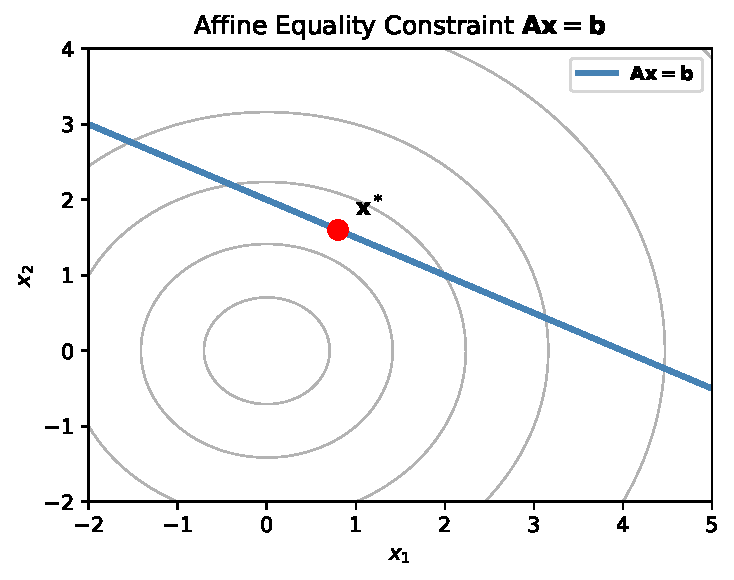
\includegraphics[width=\linewidth]{affine_equality.pdf}
      \begin{center}
        \scriptsize The constraint $x_1 + 2x_2 = 4$ (dashed line) forces
        the optimum onto the line.  The constrained minimum is
        $\bx^* = (4/5,\,8/5)$.
      \end{center}
    \end{column}
  \end{columns}

\end{frame}

\begin{frame}[fragile]{Python: Affine Equality Constraint via Substitution}
  \begin{lstlisting}[style=pycode,caption={Minimize $x_1^3+x_2^2+x_3$ subject to $x_1+2x_2+3x_3=6$ by substitution}]
import numpy as np
from scipy.optimize import minimize

# Constraint: x1 + 2*x2 + 3*x3 = 6  =>  x1 = 6 - 2*x2 - 3*x3
# We eliminate x1 and optimize over [x2, x3] only.
def f_reduced(y):
    """y = [x2, x3]; x1 is determined by the constraint."""
    x2, x3 = y
    x1 = 6.0 - 2*x2 - 3*x3
    # Original objective: x1^3 + x2^2 + x3  (substituted)
    return x1**3 + x2**2 + x3

x0 = [1.0, 1.0]
res = minimize(f_reduced, x0, method='L-BFGS-B')
x2_opt, x3_opt = res.x
x1_opt = 6.0 - 2*x2_opt - 3*x3_opt

print(f"x* = ({x1_opt:.4f}, {x2_opt:.4f}, {x3_opt:.4f})")
print(f"Constraint satisfied: {np.isclose(x1_opt + 2*x2_opt + 3*x3_opt, 6)}")
  \end{lstlisting}
\end{frame}

% =============================================================================
\section{Projected Iterative Methods}
% =============================================================================

\begin{frame}[allowframebreaks]{Projected Gradient Descent --- Staying Feasible at Every Step}

  When the feasible set $\mathcal{X}$ is a convex set (such as a box or a
  half-space), a natural extension of gradient descent is the
  \textbf{projected gradient descent} algorithm.  The key idea is:
  \begin{enumerate}
    \item Take a normal gradient step (which might leave the feasible set).
    \item \textbf{Project} the new point back onto $\mathcal{X}$ --- i.e., snap
          it to the nearest feasible point.
  \end{enumerate}
  Because both the gradient step and the projection are computable operations,
  the algorithm is simple to implement and guarantees that every iterate is
  feasible.

  \begin{block}{The Projection Operator}
    \[
      \Pi_\mathcal{X}(\tilde\bx) = \arg\min_{\bx \in \mathcal{X}}\|\bx - \tilde\bx\|_2
    \]
  \end{block}

  \begin{block}{Notation}
    \begin{itemize}
      \item $\Pi_\mathcal{X}$ (Pi sub X, where $\Pi$ is capital pi) denotes the
            \textbf{projection} operator onto $\mathcal{X}$.
      \item $\tilde\bx$ (x-tilde) is the \textbf{tentative} point --- the result
            of the gradient step, which may be infeasible.
      \item $\|\bx - \tilde\bx\|_2$ (norm of x minus x-tilde) is the Euclidean
            distance between two points.
      \item The projection finds the point in $\mathcal{X}$ that is
            \emph{closest} (in Euclidean distance) to $\tilde\bx$.
    \end{itemize}
  \end{block}

  \framebreak

  \begin{alertblock}{How to Read the Projection Formula}
    Think of $\Pi_\mathcal{X}(\tilde\bx)$ as the answer to: ``If I am standing
    at $\tilde\bx$ (which might be outside the allowed region), what is the
    closest feasible point?''  For a box constraint $[a_i, b_i]$ on each
    component, the answer is simply to \textbf{clip} each coordinate:
    $x_i = \max(a_i, \min(b_i, \tilde{x}_i))$.  For more complex sets, finding
    the projection requires solving a small quadratic program (QP).
  \end{alertblock}

  \begin{block}{Algorithm 10.1 --- Projected Gradient Descent}
    \begin{enumerate}
      \item Choose a feasible starting point $\bx^{(1)} \in \mathcal{X}$.
            (Here $\bx^{(1)}$ means $\bx$ superscript 1, the value at
            iteration 1.)
      \item At iteration $k$ (kay), compute the \textbf{gradient step}:
            \[
              \tilde{\bx} \leftarrow \bx^{(k)} - \alpha\,\nabla f\!\bigl(\bx^{(k)}\bigr)
            \]
            where $\alpha$ (alpha) is the step size (a small positive number)
            and $\nabla f$ ($\nabla$ is nabla, meaning gradient) is the vector
            of partial derivatives of $f$.
      \item \textbf{Project} back into $\mathcal{X}$:
            \[
              \bx^{(k+1)} \leftarrow \Pi_\mathcal{X}(\tilde\bx)
            \]
      \item Repeat steps 2--3 until $\|\bx^{(k+1)} - \bx^{(k)}\|$ is smaller
            than a convergence tolerance.
    \end{enumerate}
  \end{block}

  \framebreak

  \begin{columns}
    \begin{column}{0.52\textwidth}
      \begin{exampleblock}{Special cases for the projection step}
        \textbf{Box constraint} $[\mathbf{a}, \mathbf{b}]$: the projection is
        componentwise clipping,
        \[
          \bigl[\Pi_{[\mathbf{a},\mathbf{b}]}(\tilde\bx)\bigr]_i
            = \max(a_i,\, \min(b_i,\, \tilde{x}_i)).
        \]
        This is $O(n)$ (order n) --- linear in the number of variables.

        \medskip
        \textbf{Half-space} $\{\bx : \mathbf{c}^\top \bx \le d\}$
        (c bold transpose x $\le$ d): if $\tilde\bx$ violates the constraint,
        shift it back along the constraint normal $\mathbf{c}$:
        \[
          \Pi(\tilde\bx) = \tilde\bx
            - \frac{(\mathbf{c}^\top\tilde\bx - d)}{\|\mathbf{c}\|^2}\,\mathbf{c}.
        \]

        \textbf{General convex set:} solve a small QP (quadratic program) at
        each iteration.
      \end{exampleblock}
    \end{column}
    \begin{column}{0.46\textwidth}
      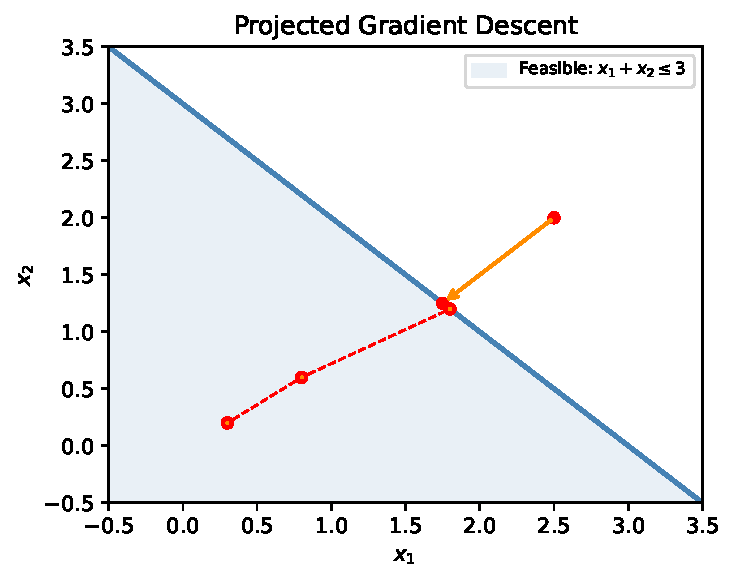
\includegraphics[width=\linewidth]{projected_descent.pdf}
      \begin{center}
        \scriptsize Orange arrows: unconstrained gradient steps that move
        outside the feasible region.  Red path: the projected iterates,
        which walk along the constraint boundary toward the constrained
        minimum.
      \end{center}
    \end{column}
  \end{columns}

  \begin{alertblock}{Key Insight}
    Projected gradient descent guarantees that \emph{every} iterate is
    feasible, which is useful when the objective or constraints are undefined
    outside $\mathcal{X}$.  The price is the projection step, which itself
    requires solving an optimization sub-problem for non-trivial sets.
  \end{alertblock}

\end{frame}

\begin{frame}[fragile]{Python: Projected Gradient Descent}
  \begin{lstlisting}[style=pycode,caption={Projected gradient descent onto the half-space $x_1 + x_2 \le 3$}]
import numpy as np

def project_halfspace(x, a, b_val):
    """Project x onto the half-space {x : a^T x <= b_val}.
    If x already satisfies the constraint, it is returned unchanged.
    Otherwise, x is shifted back onto the boundary along direction a."""
    violation = a @ x - b_val   # positive means infeasible
    if violation > 0:
        x = x - violation * a / (a @ a)
    return x

def f(x):      return (x[0]-3)**2 + (x[1]-3)**2
def grad_f(x): return np.array([2*(x[0]-3), 2*(x[1]-3)])

a = np.array([1.0, 1.0])   # constraint normal vector
b_val = 3.0                 # constraint right-hand side
x = np.array([2.5, 2.0])   # starting point (infeasible)
alpha = 0.1                 # step size (alpha)

for _ in range(50):
    x_new = x - alpha * grad_f(x)        # gradient step
    x = project_halfspace(x_new, a, b_val)  # project back

print(f"x* = {x},  constraint satisfied: {a @ x <= b_val + 1e-8}")
# x* approximately [1.5, 1.5],  constraint satisfied: True
  \end{lstlisting}
\end{frame}

% =============================================================================
\section{Lagrange Multipliers \& KKT Conditions}
% =============================================================================

\begin{frame}[allowframebreaks]{Lagrange Multipliers --- the Geometry of Equality Constraints}

  When a constraint $h(\bx) = 0$ is present, the optimal point $\bx^*$ must
  satisfy a special geometric condition: the \textbf{gradient of the objective}
  must be \textbf{parallel} to the \textbf{gradient of the constraint}.
  Intuitively, if $\nabla f(\bx^*)$ had a component \emph{along} the
  constraint surface, we could move a tiny distance along the surface
  (remaining feasible) and decrease $f$ --- contradicting optimality.

  \begin{block}{First-Order Optimality Condition for One Equality Constraint (Eq.~10.15)}
    \[
      \nabla f(\bx^*) = \lambda\,\nabla h(\bx^*)
    \]
  \end{block}

  \begin{block}{Notation}
    \begin{itemize}
      \item $\nabla f(\bx^*)$ ($\nabla$ is nabla, meaning gradient) is the
            vector of partial derivatives of $f$ evaluated at the optimal point
            $\bx^*$.  It points in the direction of steepest increase of $f$.
      \item $\nabla h(\bx^*)$ is the gradient of the constraint function $h$
            at $\bx^*$.  It is perpendicular to the constraint surface
            $h(\bx) = 0$.
      \item $\lambda$ (lambda) is the \textbf{Lagrange multiplier} --- a scalar
            that records how much the constraint gradient must be ``stretched''
            to match the objective gradient.  Its sign and magnitude convey
            economic information (the ``shadow price'' of relaxing the
            constraint by one unit).
    \end{itemize}
  \end{block}

  \framebreak

  \textbf{The Lagrangian function.}  Rather than working with the geometric
  condition directly, it is more convenient to define a single scalar function
  whose unconstrained critical points encode \emph{both} the optimality
  condition and the constraint.

  \begin{block}{The Lagrangian (Eq.~10.16)}
    \[
      \Lagr(\bx, \lambda) = f(\bx) - \lambda\,h(\bx)
    \]
  \end{block}

  \begin{block}{Notation and How to Read This}
    \begin{itemize}
      \item $\Lagr$ (script L, called the ``Lagrangian'') is a function of
            \emph{both} $\bx$ and $\lambda$ (lambda).
      \item Setting the partial derivative with respect to $\bx$ to zero,
            $\nabla_\bx \Lagr = \mathbf{0}$, gives the condition
            $\nabla f(\bx) = \lambda \nabla h(\bx)$ --- exactly the optimality
            condition above.
      \item Setting the partial derivative with respect to $\lambda$ (lambda)
            to zero, $\partial \Lagr / \partial \lambda = 0$, gives
            $h(\bx) = 0$ --- i.e., it \emph{enforces the constraint}.
    \end{itemize}
    In other words, solving the unconstrained problem
    $\nabla \Lagr(\bx, \lambda) = \mathbf{0}$ simultaneously finds the optimal
    $\bx^*$ and the Lagrange multiplier $\lambda^*$.
  \end{block}

  \framebreak

  \begin{columns}
    \begin{column}{0.55\textwidth}
      \begin{exampleblock}{Example 10.4 --- Numerical Lagrange Multiplier Solution}
        Problem:
        \[
          \min_\bx\; -\exp\!\Bigl(-\bigl(x_1 x_2 - \tfrac{3}{2}\bigr)^2
                            - \bigl(x_2 - \tfrac{3}{2}\bigr)^2\Bigr)
          \quad \text{s.t.}\quad x_1 - x_2^2 = 0.
        \]
        The Lagrangian is:
        \[
          \Lagr = -\exp(\cdots) - \lambda\,(x_1 - x_2^2).
        \]
        Setting all partial derivatives of $\Lagr$ to zero and solving
        numerically yields:
        \[
          \bx^* \approx [1.358,\; 1.165], \qquad \lambda^* \approx 0.170.
        \]
        The positive $\lambda^*$ (lambda star) means that relaxing the
        constraint (allowing $x_1 - x_2^2$ to be slightly positive) would
        improve the objective by approximately $0.170$ per unit of relaxation.
      \end{exampleblock}
    \end{column}
    \begin{column}{0.43\textwidth}
      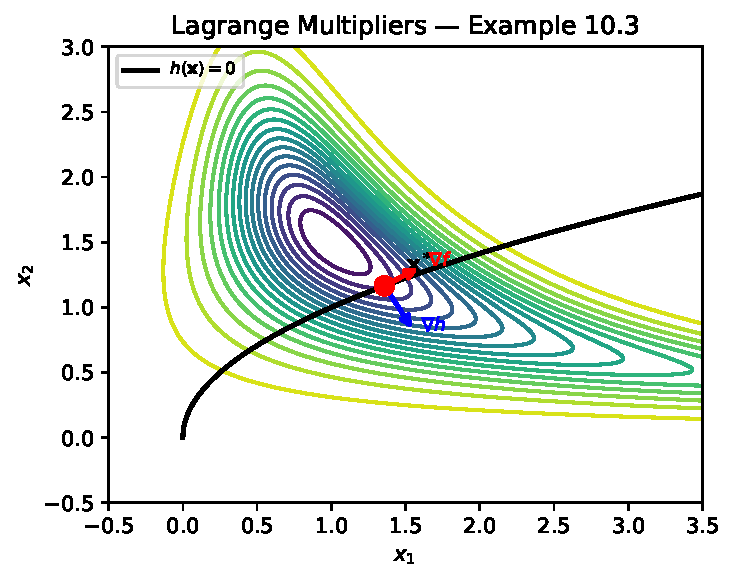
\includegraphics[width=\linewidth]{lagrange_contour.pdf}
      \begin{center}
        \scriptsize At $\bx^* \approx [1.358, 1.165]$, a level curve (contour)
        of $f$ is tangent to the constraint curve $x_1 = x_2^2$.  Tangency
        means the gradients $\nabla f$ and $\nabla h$ are parallel.
      \end{center}
    \end{column}
  \end{columns}

\end{frame}

\begin{frame}[allowframebreaks]{Multiple Equality Constraints}

  When there are $\ell$ (ell) equality constraints $h_1(\bx) = 0, \ldots,
  h_\ell(\bx) = 0$, we introduce one Lagrange multiplier $\lambda_i$ (lambda
  sub i) for each constraint.

  \begin{block}{Generalized Lagrangian for Multiple Equalities}
    \[
      \Lagr(\bx, \blambda) = f(\bx) - \sum_{i=1}^{\ell} \lambda_i\,h_i(\bx)
    \]
    where $\blambda = (\lambda_1, \ldots, \lambda_\ell)$ (lambda bold) is the
    vector of all Lagrange multipliers.
  \end{block}

  \begin{block}{Notation}
    \begin{itemize}
      \item $\sum_{i=1}^{\ell}$ (Sigma from $i=1$ to $\ell$) denotes the sum
            of $\ell$ terms.  Each term $\lambda_i h_i(\bx)$ is the product of
            multiplier $i$ and constraint function $i$.
      \item Setting $\nabla_\bx \Lagr = \mathbf{0}$ yields the stationarity
            condition:
            \[
              \nabla f(\bx) = \sum_{i=1}^{\ell} \lambda_i\,\nabla h_i(\bx),
            \]
            which says that $\nabla f$ must lie in the span (linear combination)
            of the constraint gradients.
      \item Setting $\partial \Lagr / \partial \lambda_i = 0$ for each $i$
            enforces $h_i(\bx) = 0$ for each constraint separately.
    \end{itemize}
  \end{block}

  \begin{alertblock}{How to Read the Stationarity Condition}
    The condition $\nabla f = \sum_i \lambda_i \nabla h_i$ generalises the
    single-constraint case.  It says: at an optimal point, the gradient of the
    objective can be ``explained'' as a weighted combination of the constraint
    gradients.  If this fails --- i.e., if $\nabla f$ has a component that
    cannot be expressed as such a combination --- then we could improve $f$
    while remaining feasible, contradicting optimality.
  \end{alertblock}

\end{frame}

\begin{frame}[fragile]{Python: Method of Lagrange Multipliers (Numerical)}
  \begin{lstlisting}[style=pycode,caption={Solve the KKT system for Example 10.4 using fsolve --- find x* and lambda*}]
import numpy as np
from scipy.optimize import fsolve

def f(x):
    """Objective: -exp(-(x1*x2 - 3/2)^2 - (x2 - 3/2)^2)"""
    return -np.exp(-((x[0]*x[1] - 1.5)**2 + (x[1] - 1.5)**2))

def grad_L(vars):
    """Gradient of the Lagrangian L(x1, x2, lambda) = f(x) - lambda*(x1 - x2^2).
    We set all three partial derivatives to zero and solve the system."""
    x1, x2, lam = vars
    fval = f([x1, x2])
    # dL/dx1: derivative of f w.r.t. x1 minus lambda*(d/dx1)(x1 - x2^2)
    dLdx1 = 2*x2*fval*(x1*x2 - 1.5) - lam
    # dL/dx2: derivative of f w.r.t. x2 minus lambda*(d/dx2)(x1 - x2^2)
    dLdx2 = 2*lam*x2*fval + fval*(-2*x1*(x1*x2-1.5) - 2*(x2-1.5))
    # dL/dlambda: enforces the constraint h(x) = x1 - x2^2 = 0
    dLdlam = -(x2**2 - x1)
    return [dLdx1, dLdx2, dLdlam]

x0 = [1.0, 1.0, 0.1]          # initial guess for (x1, x2, lambda)
sol = fsolve(grad_L, x0, full_output=True)
x1s, x2s, lams = sol[0]
print(f"x* = [{x1s:.4f}, {x2s:.4f}],  lambda* = {lams:.4f}")
# x* = [1.3580, 1.1650],  lambda* = 0.1700
  \end{lstlisting}
\end{frame}

% =============================================================================
\section{Inequality Constraints \& KKT Conditions}
% =============================================================================

\begin{frame}[allowframebreaks]{KKT Conditions --- the Full First-Order Theory}

  The Lagrange multiplier theory extends elegantly to inequality constraints
  $g_j(\bx) \le 0$ by introducing one multiplier $\mu_j$ (mu sub j) per
  inequality.  The resulting \textbf{Karush-Kuhn-Tucker (KKT) conditions} are
  the first-order necessary conditions for a constrained minimum of any
  smooth problem.

  \begin{block}{Generalized Lagrangian with Equality and Inequality Constraints}
    \[
      \Lagr(\bx, \blambda, \bmu)
        = f(\bx)
          - \sum_{i=1}^{\ell} \lambda_i h_i(\bx)
          - \sum_{j=1}^{m} \mu_j g_j(\bx)
    \]
  \end{block}

  \begin{block}{Notation}
    \begin{itemize}
      \item $\blambda = (\lambda_1, \ldots, \lambda_\ell)$ (lambda bold) are
            the multipliers for the $\ell$ equality constraints; they are
            \emph{unrestricted} in sign.
      \item $\bmu = (\mu_1, \ldots, \mu_m)$ (mu bold) are the multipliers for
            the $m$ inequality constraints; they must be
            \textbf{non-negative} ($\mu_j \ge 0$) --- this is the dual feasibility
            condition explained below.
      \item $\sum_{j=1}^{m}$ (Sigma from $j=1$ to $m$) sums over all $m$
            inequality constraints.
    \end{itemize}
  \end{block}

  \framebreak

  \begin{block}{The Four KKT Necessary Conditions}
    At any local minimum $\bx^*$ (under a constraint qualification):
    \begin{enumerate}
      \item \textbf{Stationarity:} $\nabla_\bx \Lagr(\bx^*, \blambda^*, \bmu^*) = \mathbf{0}$.
            The gradient of the Lagrangian with respect to $\bx$ (x bold) must
            be zero, just as in unconstrained optimization.

      \item \textbf{Primal feasibility:} $h_i(\bx^*) = 0$ for all $i$, and
            $g_j(\bx^*) \le 0$ for all $j$.  The optimal point must satisfy
            all constraints.

      \item \textbf{Dual feasibility:} $\mu_j^* \ge 0$ for all $j$.  The
            multipliers for inequality constraints must be non-negative.  This
            ensures that the constraint gradient pushes the objective in the
            correct direction (into the feasible set).

      \item \textbf{Complementary slackness:} $\mu_j^*\, g_j(\bx^*) = 0$ for
            all $j$.  For each inequality, \emph{either} the multiplier is zero
            \emph{or} the constraint is tight (equals zero), but both cannot be
            non-zero simultaneously.
    \end{enumerate}
  \end{block}

  \framebreak

  \begin{columns}
    \begin{column}{0.55\textwidth}
      \begin{alertblock}{How to Read Complementary Slackness}
        The condition $\mu_j g_j(\bx^*) = 0$ encodes the two possible
        situations at an optimal point:

        \begin{itemize}
          \item \textbf{Inactive constraint} ($g_j(\bx^*) < 0$): the point is
                strictly inside the feasible set.  Then $\mu_j^* = 0$; the
                constraint has no influence on the solution.

          \item \textbf{Active constraint} ($g_j(\bx^*) = 0$): the point sits
                exactly on the boundary.  Then $\mu_j^* > 0$; the constraint is
                ``binding'' and pulls the solution to the boundary.
        \end{itemize}

        The product of these two quantities must always be zero: if $g_j < 0$,
        we need $\mu_j = 0$; if $\mu_j > 0$, we need $g_j = 0$.
      \end{alertblock}
    \end{column}
    \begin{column}{0.43\textwidth}
      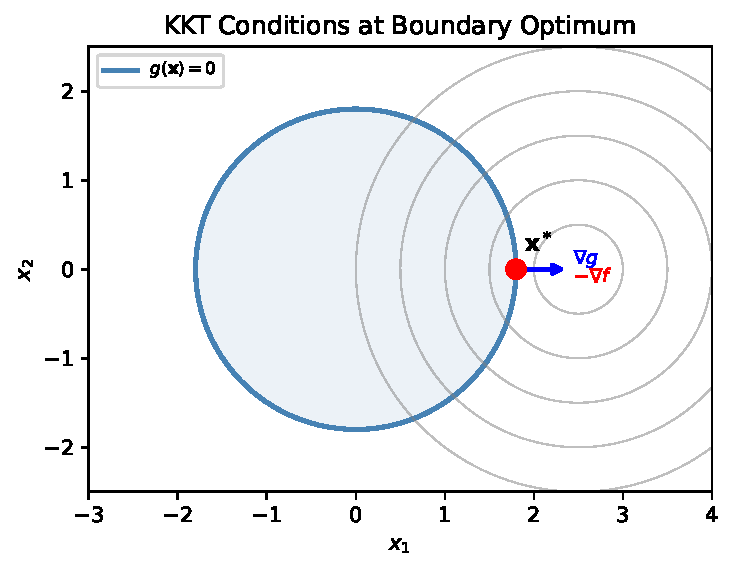
\includegraphics[width=\linewidth]{kkt_conditions.pdf}
      \begin{center}
        \scriptsize At a boundary optimum: $-\nabla f$ and $\nabla g$ are
        aligned ($\mu^* > 0$).  At an interior optimum: the constraint
        gradient is not needed ($\mu^* = 0$).
      \end{center}
    \end{column}
  \end{columns}

\end{frame}

\begin{frame}[allowframebreaks]{Active vs.\ Inactive Constraints --- Worked Intuition}

  Understanding whether a constraint is active or inactive at the solution is
  crucial for selecting efficient algorithms.  The distinction maps directly
  onto the complementary slackness KKT condition.

  \begin{columns}
    \begin{column}{0.50\textwidth}
      \begin{block}{Inactive Constraint --- $g(\bx^*) < 0$}
        When the unconstrained minimum already satisfies $g(\bx^*) < 0$
        (strictly inside the feasible region), the constraint has no effect on
        the solution.  The KKT condition forces $\mu_j^* = 0$, meaning the
        corresponding multiplier is zero.  Locally, the problem behaves
        exactly like an unconstrained one.
      \end{block}

      \begin{block}{Active Constraint --- $g(\bx^*) = 0$}
        When the unconstrained minimum is infeasible (i.e., $g(\bx) < 0$ is
        violated at the unconstrained optimum), the constrained minimum is
        forced to the boundary $g(\bx^*) = 0$.  The KKT condition gives
        $\mu_j^* > 0$, meaning the constraint is ``binding'': the gradient of
        $f$ at $\bx^*$ has a component pointing into the infeasible region,
        and the constraint gradient exactly cancels it.
      \end{block}
    \end{column}
    \begin{column}{0.48\textwidth}
      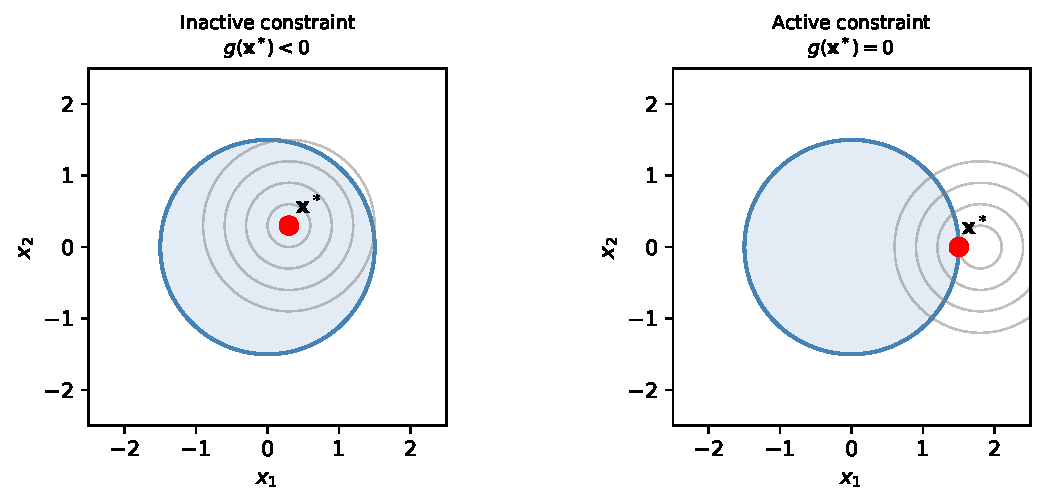
\includegraphics[width=\linewidth]{inequality_region.pdf}
      \begin{center}
        \scriptsize Left panel: the unconstrained minimum lies inside the
        feasible region, so the constraint is inactive ($\mu = 0$).  Right
        panel: the minimum lies outside the feasible region, so it moves to
        the boundary (active constraint, $\mu > 0$).
      \end{center}
    \end{column}
  \end{columns}

  \begin{alertblock}{Key Insight}
    At an optimal point, each inequality constraint is either \emph{on} or
    \emph{off}: either it is active and pushing the solution to the boundary,
    or it is inactive and irrelevant.  This binary behaviour is exploited by
    \textbf{active-set methods}, which maintain a working set of active
    constraints and update it as the algorithm progresses.
  \end{alertblock}

\end{frame}

% =============================================================================
\section{Slack Variables}
% =============================================================================

\begin{frame}[allowframebreaks]{Slack Variables --- Converting Inequalities to Equalities}

  A \textbf{slack variable} is a device that converts an inequality constraint
  into an equality constraint by absorbing the ``slack'' --- the gap between
  the left-hand side and zero.  This is useful because some methods (e.g.,
  Lagrange multipliers, the method of multipliers) are designed for equality
  constraints only.

  \begin{block}{The Slack Variable Trick}
    Given an inequality $g(\bx) \le 0$, introduce a new variable $s \ge 0$
    (the slack) so that:
    \[
      g(\bx) + s = 0, \qquad s \ge 0.
    \]
    The slack $s$ measures how far the constraint is from being tight:
    if $s = 0$, the constraint is active; if $s > 0$, the constraint is
    inactive with slack $s$.
  \end{block}

  The remaining problem is: how do we enforce $s \ge 0$ without another
  inequality constraint?  We use a further substitution $s = t^2$, where
  $t \in \R$ is unconstrained.  Then $s = t^2 \ge 0$ automatically.

  \begin{block}{Full Transformation (no constraints on new variables)}
    \[
      g(\bx) + t^2 = 0, \qquad t \in \R \text{ (unconstrained)}.
    \]
    The original inequality $g(\bx) \le 0$ has been converted to an equality
    constraint involving both $\bx$ and the new variable $t$.
  \end{block}

  \framebreak

  \begin{columns}
    \begin{column}{0.52\textwidth}
      \textbf{Procedure for $m$ inequality constraints.}  Introduce $m$
      unconstrained variables $t_1, t_2, \ldots, t_m$ and replace each
      $g_j(\bx) \le 0$ by:
      \[
        g_j(\bx) + t_j^2 = 0, \quad j = 1, \ldots, m.
      \]
      The augmented problem has $n + m$ variables (the original $n$ plus $m$
      new ones) and $m$ equality constraints.

      \begin{block}{Transformed Problem}
        \[
          \minimize_{\bx,\,t_1,\ldots,t_m}\; f(\bx)
          \quad\text{s.t.}\quad
          g_j(\bx) + t_j^2 = 0\;\;\forall j
        \]
        This is now a \textbf{pure equality}-constrained problem,
        amenable to Lagrange multiplier methods.
      \end{block}
    \end{column}
    \begin{column}{0.46\textwidth}
      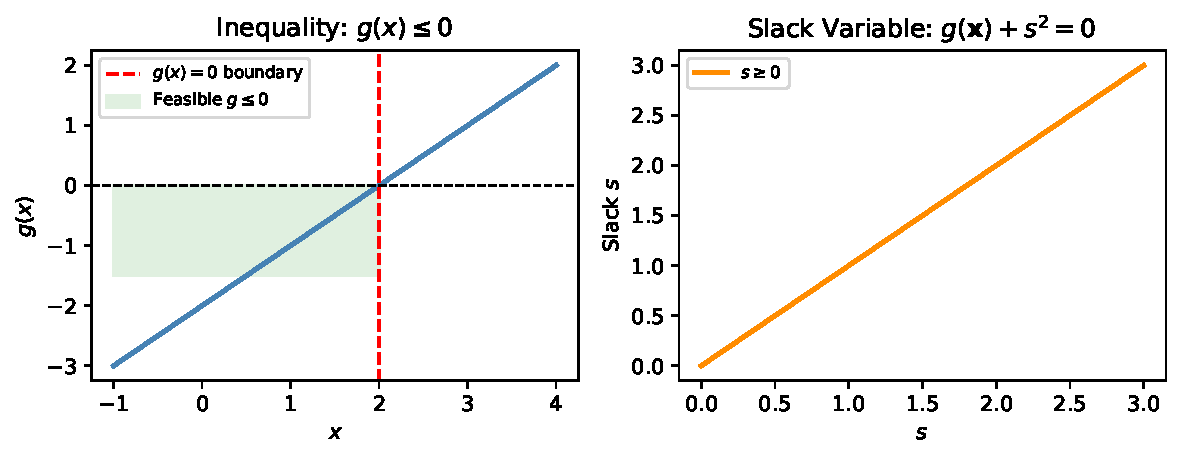
\includegraphics[width=\linewidth]{slack_variable.pdf}
      \begin{center}
        \scriptsize The slack $s = t^2 \ge 0$ ``absorbs'' the gap between
        $g(\bx)$ and zero, converting the one-sided constraint into an exact
        equality.
      \end{center}

      \begin{exampleblock}{Worked Example}
        Constraint: $g(x) = x - 5 \le 0$.

        \medskip
        Introduce $t \in \R$, set $g(x) + t^2 = 0$:
        \[
          x - 5 + t^2 = 0 \;\Longrightarrow\; x = 5 - t^2 \le 5.\ \checkmark
        \]
        For any real $t$, we get $x \le 5$ automatically.
      \end{exampleblock}
    \end{column}
  \end{columns}

  \begin{alertblock}{Key Insight}
    Slack variables do \emph{not} reduce the difficulty of the problem --- they
    merely change its form.  The real benefit is that standard equality-only
    methods (Lagrange multipliers, augmented Lagrangian) can now be applied
    without modification.
  \end{alertblock}

\end{frame}

% =============================================================================
\section{Penalty Methods}
% =============================================================================

\begin{frame}[allowframebreaks]{Penalty Methods --- Enforcing Constraints by Adding a Cost}

  A \textbf{penalty method} converts a constrained problem into a sequence of
  unconstrained problems by adding a term to the objective that is large
  whenever the constraints are violated.  The intuition is: if violating
  a constraint costs a lot, the optimizer will try hard to avoid violations.
  As we increase the cost (the penalty weight $\rho$ (rho)), the optimizer
  is forced closer and closer to feasibility.

  \begin{block}{Penalized Objective}
    \[
      \minimize_{\bx}\; f(\bx) + \rho\,p(\bx)
    \]
  \end{block}

  \begin{block}{Notation and How to Read This}
    \begin{itemize}
      \item $\rho$ (rho) is the \textbf{penalty weight} (a positive scalar that
            controls how severely constraint violations are penalized).  Small
            $\rho$ allows mild violations; large $\rho$ forces near-feasibility.
      \item $p(\bx)$ is the \textbf{penalty function} --- a non-negative
            function that equals zero when all constraints are satisfied and
            is positive when constraints are violated.
    \end{itemize}
    Reading this formula: the optimizer minimizes both $f(\bx)$ (the original
    goal) and $\rho\, p(\bx)$ (the penalty for infeasibility).  These two
    terms trade off against each other: if $\rho$ is too small, the penalty is
    weak and the solution may be infeasible; if $\rho$ is too large, the
    problem becomes ill-conditioned.
  \end{block}

  \framebreak

  There are several natural choices for the penalty function $p(\bx)$, each
  with different properties.

  \begin{block}{Common Penalty Functions}
    \begin{itemize}
      \item \textbf{Count penalty:} $p(\bx) = \sum_j \mathbf{1}[g_j(\bx) > 0]$
            counts the number of violated constraints.  Each violation adds 1
            to the penalty regardless of severity.  This is \emph{non-smooth}
            (non-differentiable) and hard to optimize with gradient methods.

      \item \textbf{Quadratic penalty (for inequalities):}
            $p(\bx) = \sum_j \max(g_j(\bx), 0)^2$.
            Only the \emph{violated} constraints (where $g_j > 0$) contribute,
            and the contribution grows as the \emph{square} of the violation.
            This is smooth everywhere.

      \item \textbf{Quadratic penalty (for equalities):}
            $p(\bx) = \sum_i h_i(\bx)^2$.
            Since $h_i(\bx)^2 \ge 0$ and equals zero iff $h_i(\bx) = 0$,
            this penalises any deviation from the equality surface.
    \end{itemize}
  \end{block}

  \begin{columns}
    \begin{column}{0.52\textwidth}
      \textbf{Sequential penalty strategy.}  Rather than using a single large
      $\rho$, it is better to solve a sequence of sub-problems with
      \emph{increasing} $\rho$:
      \[
        \rho_1 < \rho_2 < \cdots \to \infty.
      \]
      At each stage, the solution from the previous stage initialises the next.
      This warm-starting approach converges more reliably than starting from
      scratch each time.
    \end{column}
    \begin{column}{0.46\textwidth}
      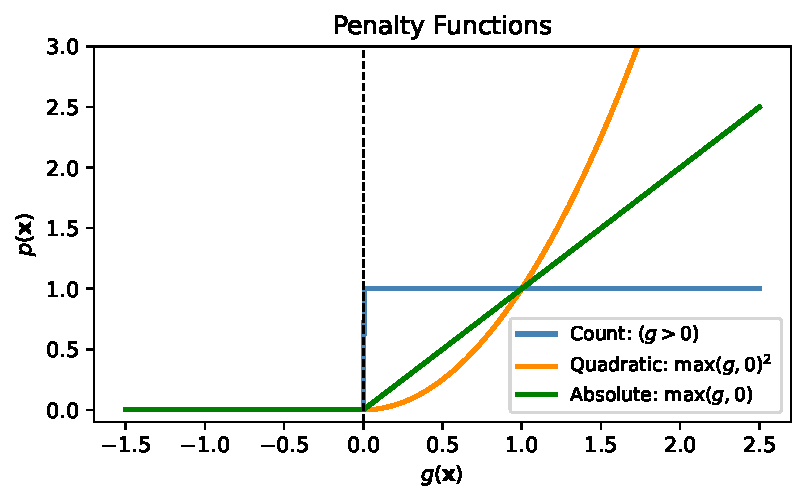
\includegraphics[width=\linewidth]{penalty_functions.pdf}
      \begin{center}
        \scriptsize Different penalty functions plotted as a function of the
        constraint value $g(\bx)$.  The quadratic penalty (blue curve) grows
        smoothly, while the count penalty (step function) is non-differentiable.
      \end{center}
    \end{column}
  \end{columns}

  \framebreak

  \begin{columns}
    \begin{column}{0.52\textwidth}
      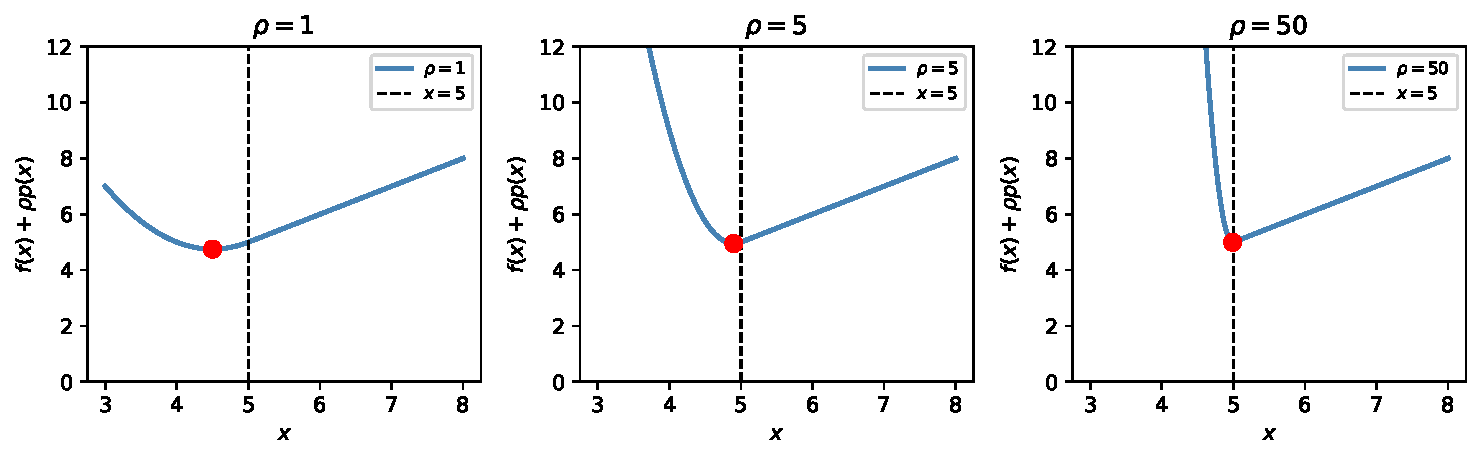
\includegraphics[width=\linewidth]{penalty_method_rho.pdf}
      \begin{center}
        \scriptsize Penalized objective for $\min x$ subject to $x \ge 5$,
        for increasing values of $\rho$.  The minimum $x^* = 5 - 1/(2\rho)$
        (x star equals 5 minus one over two rho) approaches 5 from below as
        $\rho \to \infty$.
      \end{center}
    \end{column}
    \begin{column}{0.46\textwidth}
      \begin{alertblock}{Key Limitation (Example 10.5)}
        For the problem $\min\, x$ subject to $x \ge 5$, the penalized
        problem (with quadratic penalty for $x < 5$) has the closed-form
        unconstrained minimum:
        \[
          x^* = 5 - \frac{1}{2\rho}.
        \]
        This value is always \emph{strictly less than 5} for any finite $\rho$
        (rho): the solution never actually reaches the constraint boundary.
        Exact feasibility requires $\rho \to \infty$, which causes the Hessian
        (second-derivative matrix) to become ill-conditioned and the solver to
        slow dramatically.
      \end{alertblock}

      \begin{block}{Practical issues with large $\rho$}
        As $\rho$ grows, the penalized objective develops a very ``steep
        valley'' near the constraint boundary.  The condition number of the
        Hessian grows, gradient steps become tiny, and convergence stalls.
        This is the principal weakness of pure penalty methods.
      \end{block}
    \end{column}
  \end{columns}

\end{frame}

\begin{frame}[fragile]{Python: Quadratic Penalty Method}
  \begin{lstlisting}[style=pycode,caption={Quadratic penalty method for equality-constrained minimization}]
import numpy as np
from scipy.optimize import minimize

def quadratic_penalty_method(f, h, x0, k_max=20, rho=1.0, gamma=2.0):
    """
    Minimize f(x) subject to h(x) = 0 using quadratic penalty.
    f    : objective function
    h    : equality constraint function (returns array)
    x0   : initial point
    k_max: number of penalty iterations (outer loop)
    rho  : initial penalty weight (rho, pronounced 'row')
    gamma: factor by which rho is multiplied each iteration (> 1)
    """
    x = np.array(x0, dtype=float)
    for k in range(k_max):
        def penalized(xv):
            hv = h(xv)
            # Penalized objective: f(x) + (rho/2) * ||h(x)||^2
            return f(xv) + (rho / 2.0) * np.sum(hv**2)
        res = minimize(penalized, x, method='L-BFGS-B')
        x = res.x
        rho *= gamma    # increase penalty weight for next iteration
    return x

# Example: minimize x1^2 + x2^2 subject to x1 + x2 = 1
# True solution: x* = [0.5, 0.5] (closest point on the line to the origin)
f  = lambda x: x[0]**2 + x[1]**2
h  = lambda x: np.array([x[0] + x[1] - 1.0])
x_opt = quadratic_penalty_method(f, h, [0.5, 0.5])
print(f"x* = {x_opt}")   # x* approximately [0.5, 0.5]
  \end{lstlisting}
\end{frame}

% =============================================================================
\section{Method of Multipliers (Augmented Lagrangian)}
% =============================================================================

\begin{frame}[allowframebreaks]{Method of Multipliers --- The Best of Both Worlds}

  The \textbf{method of multipliers} (also called the \textbf{augmented
  Lagrangian method}) fixes the key weakness of the pure penalty method by
  combining a quadratic penalty with an estimate of the true Lagrange
  multiplier.  The key insight is: if we had the \emph{exact} multiplier
  $\lambda^*$, the augmented Lagrangian $\Lagr_\rho$ would have its
  unconstrained minimum \emph{exactly} at the constrained optimum $\bx^*$,
  even for a \emph{finite} value of $\rho$.  The method iteratively refines
  the multiplier estimate using a simple update rule.

  \begin{block}{Augmented Lagrangian Function (Eq.~10.37)}
    \[
      \Lagr_\rho(\bx, \blambda)
        = f(\bx)
          + \frac{\rho}{2}\,\|\mathbf{h}(\bx)\|^2
          + \blambda^\top \mathbf{h}(\bx)
    \]
  \end{block}

  \begin{block}{Notation and How to Read This}
    \begin{itemize}
      \item $\rho$ (rho) is the penalty weight (a positive scalar), same role as
            in the pure penalty method.
      \item $\mathbf{h}(\bx) = (h_1(\bx), \ldots, h_\ell(\bx))$ is the vector
            of all equality constraint values.
      \item $\|\mathbf{h}(\bx)\|^2$ (norm squared of h) is the sum of squares
            of the constraint values: $h_1(\bx)^2 + \cdots + h_\ell(\bx)^2$.
            This is the quadratic penalty term from the pure penalty method.
      \item $\blambda$ (lambda bold) is the current \textbf{estimate} of the
            Lagrange multiplier vector.
      \item $\blambda^\top \mathbf{h}(\bx)$ (lambda transpose times h) is
            the dot product of the multiplier estimate and the constraint vector:
            $\lambda_1 h_1(\bx) + \cdots + \lambda_\ell h_\ell(\bx)$.  This is
            the classical Lagrangian term.
    \end{itemize}
    Compared to the pure penalty method, the only difference is the added term
    $\blambda^\top \mathbf{h}(\bx)$, which shifts the penalty ``center'' so
    that the unconstrained minimum approaches the true constrained minimum at
    finite $\rho$.
  \end{block}

  \framebreak

  \begin{block}{Algorithm 10.3 --- Method of Multipliers}
    \begin{enumerate}
      \item \textbf{Initialize:} set $\blambda \leftarrow \mathbf{0}$ (zero
            multiplier estimate) and choose $\rho > 0$, $\gamma > 1$ (gamma
            is the growth factor for $\rho$).
      \item \textbf{Inner minimization:} find $\bx$ that minimizes the
            augmented Lagrangian for the current $\blambda$ and $\rho$:
            \[
              \bx \leftarrow \arg\min_{\bx}\;\Lagr_\rho(\bx, \blambda).
            \]
            This is an \emph{unconstrained} minimization and can use any
            standard solver.
      \item \textbf{Multiplier update:}
            \[
              \blambda \leftarrow \blambda + \rho\,\mathbf{h}(\bx).
            \]
            If $h(\bx) > 0$ (constraint violated), we increase $\lambda$, making
            the penalty term larger and pushing $\bx$ toward feasibility.
      \item \textbf{Increase $\rho$:} $\rho \leftarrow \gamma\rho$.
      \item \textbf{Repeat} steps 2--4 until $\|\mathbf{h}(\bx)\| \le \varepsilon$
            (epsilon), where $\varepsilon$ (epsilon) is a small convergence
            tolerance.
    \end{enumerate}
  \end{block}

  \framebreak

  \begin{columns}
    \begin{column}{0.55\textwidth}
      \begin{alertblock}{How to Read the Multiplier Update}
        The update rule $\blambda \leftarrow \blambda + \rho\,\mathbf{h}(\bx)$
        is a gradient ascent step on the dual objective.  Here is the intuition:

        \begin{itemize}
          \item If $h(\bx) > 0$ (constraint violated), then $\lambda$ increases.
                A larger $\lambda$ makes the Lagrangian penalize the violation
                more heavily, so the next minimization step moves $\bx$ closer
                to feasibility.
          \item If $h(\bx) < 0$ (constraint over-satisfied), $\lambda$ decreases,
                relaxing the penalty.
          \item At convergence, $h(\bx) = 0$ and $\blambda$ has converged to
                the true Lagrange multiplier $\blambda^*$.
        \end{itemize}

        This feedback mechanism means feasibility is achieved \emph{at finite}
        $\rho$, unlike the pure penalty method.
      \end{alertblock}
    \end{column}
    \begin{column}{0.43\textwidth}
      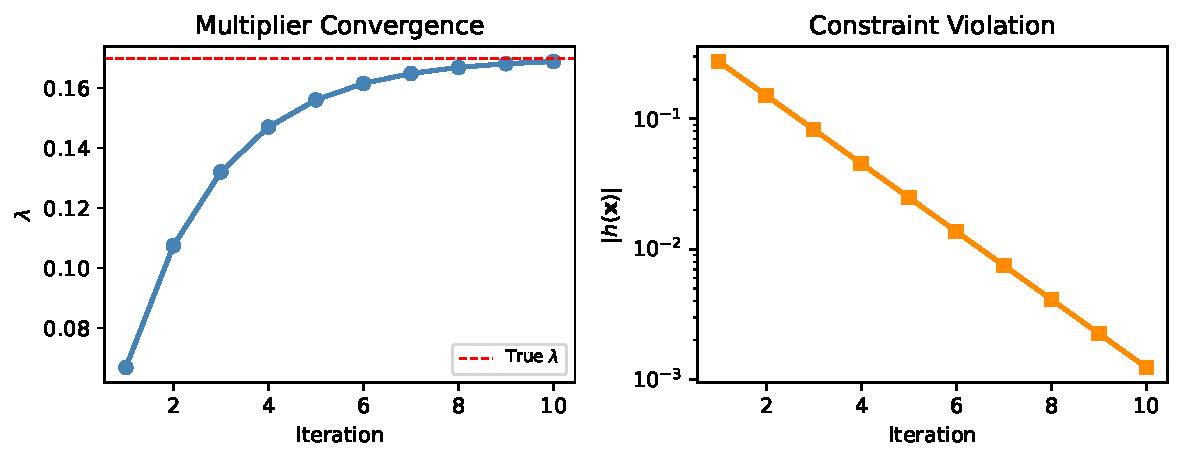
\includegraphics[width=\linewidth]{method_of_multipliers_conv.pdf}
      \begin{center}
        \scriptsize Left panel: multiplier estimate $\lambda^{(k)}$ (lambda
        superscript k) converging to the true $\lambda^*$.  Right panel:
        constraint violation $\|\mathbf{h}(\bx^{(k)})\|$ converging to zero.
      \end{center}
    \end{column}
  \end{columns}

\end{frame}

\begin{frame}[fragile]{Python: Method of Multipliers (Augmented Lagrangian)}
  \begin{lstlisting}[style=pycode,caption={Method of Multipliers (Algorithm 10.3) in Python --- equality constraints}]
import numpy as np
from scipy.optimize import minimize

def method_of_multipliers(f, h, x0, k_max=20, rho=1.0, gamma=2.0):
    """
    Minimize f(x) subject to h(x) = 0 using the augmented Lagrangian method.
    f     : objective function
    h     : equality constraint function (returns array)
    x0    : initial point
    k_max : maximum outer iterations
    rho   : initial penalty weight
    gamma : penalty growth factor (> 1)
    """
    x = np.array(x0, dtype=float)
    lam = np.zeros(len(h(x)))      # initialize Lagrange multipliers to zero
    for k in range(k_max):
        def aug_lagrangian(xv):
            hv = h(xv)
            # Augmented Lagrangian: f(x) + (rho/2)||h||^2 + lambda^T h
            return f(xv) + (rho / 2.0) * np.dot(hv, hv) + np.dot(lam, hv)
        res = minimize(aug_lagrangian, x, method='L-BFGS-B')
        x   = res.x
        lam = lam + rho * h(x)    # multiplier update: lam <- lam + rho * h(x)
        rho *= gamma              # increase penalty weight
        if np.linalg.norm(h(x)) < 1e-8:
            break
    return x, lam

# Example: minimize x1^2 + x2^2 subject to x1 + x2 = 1
f  = lambda x: x[0]**2 + x[1]**2
h  = lambda x: np.array([x[0] + x[1] - 1.0])
x_opt, lam_opt = method_of_multipliers(f, h, [2.0, 0.0])
print(f"x* = {x_opt},  lambda* = {lam_opt}")
# x* approximately [0.5, 0.5],  lambda* approximately [-1.0]
  \end{lstlisting}
\end{frame}

% =============================================================================
\section{Interior Point Methods}
% =============================================================================

\begin{frame}[allowframebreaks]{Interior Point Methods --- Staying Inside by Adding a Barrier}

  Interior point methods take the opposite philosophical approach from penalty
  methods: instead of penalizing infeasibility (staying outside), they add a
  \textbf{barrier} that prevents the optimizer from ever \emph{reaching} the
  boundary.  Every iterate is strictly feasible throughout the entire algorithm.

  \textbf{The core idea.}  For an inequality constraint $g_j(\bx) \le 0$,
  define a function that becomes $+\infty$ (plus infinity) as $g_j(\bx)$
  approaches zero from below (i.e., as $\bx$ approaches the boundary from
  the interior).  This infinite ``wall'' stops the optimizer from crossing
  the boundary.

  \begin{block}{Log Barrier for $g_j(\bx) \le 0$}
    \[
      p(\bx) = -\sum_{j=1}^{m} \ln\!\bigl(-g_j(\bx)\bigr)
    \]
    This function is defined only when all $g_j(\bx) < 0$ (i.e., strictly
    inside the feasible set).
  \end{block}

  \begin{block}{Notation and How to Read This}
    \begin{itemize}
      \item $\ln(\cdot)$ (natural logarithm) is a function that approaches
            $-\infty$ as its argument approaches zero from above.
      \item Since $g_j(\bx) < 0$ in the interior, $-g_j(\bx) > 0$, so
            $\ln(-g_j(\bx))$ is well-defined.
      \item As $g_j(\bx) \to 0^-$ (approaches zero from below), $-g_j(\bx) \to 0^+$,
            and $\ln(-g_j(\bx)) \to -\infty$.  Therefore $-\ln(-g_j(\bx)) \to +\infty$:
            the barrier blows up, creating a wall at the boundary.
      \item The sum $\sum_{j=1}^m$ (Sigma over all $m$ constraints) adds a wall
            for every inequality.
    \end{itemize}
  \end{block}

  \framebreak

  \begin{block}{Barrier-Penalized Objective}
    \[
      \minimize_{\bx}\; f(\bx) + \frac{1}{\rho}\,p(\bx)
    \]
    where $\rho > 0$ (rho) controls how ``thick'' the barrier wall is.  For
    small $\rho$ the barrier is very strong (the $1/\rho$ coefficient is large),
    keeping the solution far from the boundary.  As $\rho$ increases, the barrier
    shrinks, allowing the solution to approach the boundary.
  \end{block}

  \begin{alertblock}{How to Read This Formula}
    Increasing $\rho$ (rho) makes $1/\rho$ smaller, reducing the influence of
    the barrier.  The sequence of minimizers, as $\rho \to \infty$, traces a
    \textbf{central path} from the interior toward the constrained optimum on
    the boundary.  This central-path concept is the foundation of modern
    interior-point methods for linear and convex programs.
  \end{alertblock}

  \begin{columns}
    \begin{column}{0.52\textwidth}
      \begin{block}{Other Barrier Functions}
        \begin{itemize}
          \item \textbf{Inverse barrier:}
                $p(\bx) = -\sum_j \frac{1}{g_j(\bx)}$.
                This also blows up at the boundary but has different curvature
                properties than the log barrier.
        \end{itemize}
        Both types require a \textbf{strictly feasible} starting point
        $\bx^{(0)}$ with all $g_j(\bx^{(0)}) < 0$.
      \end{block}
    \end{column}
    \begin{column}{0.46\textwidth}
      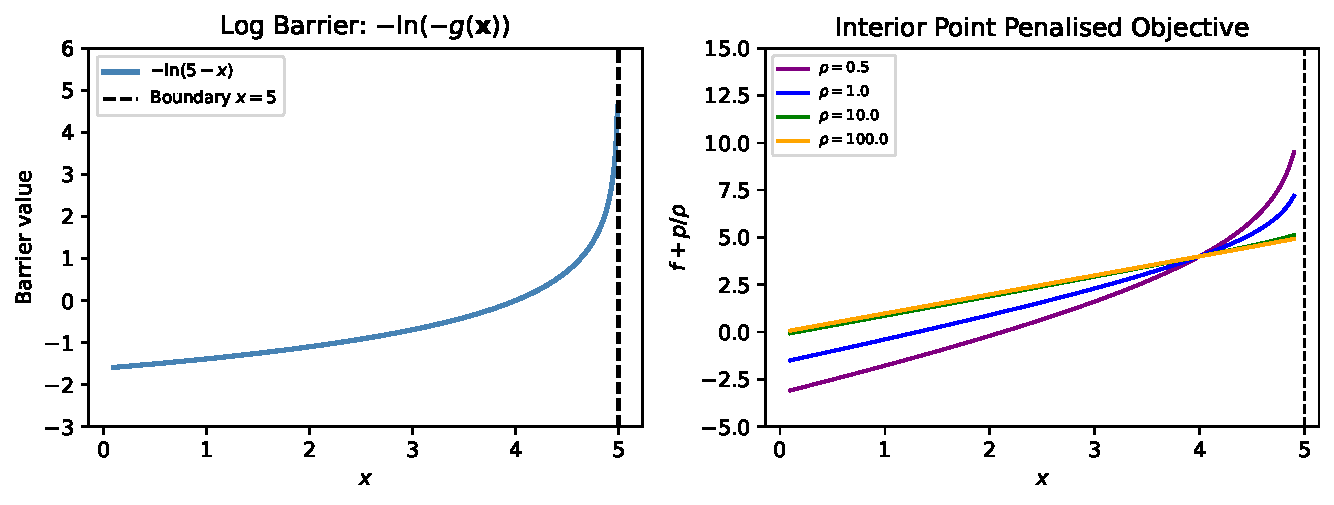
\includegraphics[width=\linewidth]{interior_point_barrier.pdf}
      \begin{center}
        \scriptsize Left: the log barrier blows up at the constraint boundary.
        Right: as $\rho$ increases, the minimizer of the barrier-penalized
        problem moves toward the boundary, tracing the central path.
      \end{center}
    \end{column}
  \end{columns}

\end{frame}

\begin{frame}[allowframebreaks]{Interior Point Algorithm and Finding a Feasible Starting Point}

  \begin{block}{Algorithm 10.4 --- Interior Point Method}
    \begin{enumerate}
      \item Choose a \textbf{strictly feasible} starting point $\bx^{(0)}$
            satisfying $g_j(\bx^{(0)}) < 0$ for all $j$ (all constraints
            strictly satisfied).
      \item Set $\delta \leftarrow \infty$ (delta, measuring the step size).
      \item \textbf{While} $\delta > \varepsilon$ (epsilon, the convergence
            threshold):
            \begin{enumerate}
              \item Minimize the barrier-penalized objective to get $\bx'$:
                    $\bx' \leftarrow \arg\min_\bx\bigl[f(\bx) + p(\bx)/\rho\bigr]$.
              \item Measure change: $\delta \leftarrow \|\bx' - \bx\|$.
              \item Update: $\bx \leftarrow \bx'$.
              \item Increase barrier: $\rho \leftarrow \gamma\rho$.
            \end{enumerate}
      \item \textbf{Return} $\bx$ as the approximate constrained minimum.
    \end{enumerate}
  \end{block}

  \textbf{Finding an initial strictly feasible point.}  If no feasible point
  is known, solve an auxiliary problem to find one:
  \[
    \minimize_{\bx,\,s}\; s
    \quad\text{s.t.}\quad
    \mathbf{g}(\bx) \le s\,\mathbf{1}
  \]
  where $\mathbf{1}$ is a vector of ones and $s$ (a scalar) is also being
  minimized.  Start with any $\bx^{(0)}$ and set
  $s^{(0)} > \max_j g_j(\bx^{(0)})$ (so the pair $(\bx^{(0)}, s^{(0)})$ is
  feasible for the auxiliary problem).  When this auxiliary problem finds
  $s^* < 0$, the corresponding $\bx^*$ is strictly feasible for the original
  problem.

  \framebreak

  \begin{columns}
    \begin{column}{0.55\textwidth}
      \begin{exampleblock}{Feasibility sub-problem explained}
        The auxiliary problem $\min\, s$ subject to $\mathbf{g}(\bx) \le s\mathbf{1}$
        asks: ``find the smallest $s$ such that all constraint violations
        are at most $s$.''  If the minimum $s^* < 0$, then
        $g_j(\bx^*) \le s^* < 0$ for all $j$, meaning $\bx^*$ is
        \emph{strictly} feasible for the original problem.  If $s^* > 0$,
        the original problem is infeasible.
      \end{exampleblock}

      \begin{block}{Pros and Cons}
        \textbf{Advantages:}
        \begin{itemize}
          \item Every iterate is strictly feasible.
          \item Works extremely well for convex problems (LP, QP, SOCP).
          \item The basis of production solvers such as IPOPT and MOSEK.
        \end{itemize}
        \textbf{Disadvantages:}
        \begin{itemize}
          \item Requires a strictly feasible starting point.
          \item The barrier becomes ill-conditioned as $\rho \to \infty$.
        \end{itemize}
      \end{block}
    \end{column}
    \begin{column}{0.43\textwidth}
      \begin{exampleblock}{Worked Example}
        Problem: $\min\,(x-3)^2$ subject to $x \ge 1$, i.e., $g(x) = 1 - x \le 0$.

        \medskip
        The unconstrained minimum is at $x = 3$, which satisfies $x \ge 1$.
        So the constraint is inactive and $x^* = 3$.

        \medskip
        Starting from $x^{(0)} = 1.5$ (strictly feasible since $1.5 > 1$),
        the interior point algorithm traces a path toward $x^* = 3$ while
        staying above $x = 1$ throughout.
      \end{exampleblock}
    \end{column}
  \end{columns}

\end{frame}

\begin{frame}[fragile]{Python: Interior Point Method with Log Barrier}
  \begin{lstlisting}[style=pycode,caption={Interior point method with log barrier for inequality constraints}]
import numpy as np
from scipy.optimize import minimize

def interior_point_method(f, g_list, x0, rho=1.0, gamma=2.0, eps=1e-6):
    """
    Minimize f(x) subject to g_j(x) <= 0 for all g in g_list.
    f       : objective function
    g_list  : list of inequality constraint functions (each g_j(x) <= 0)
    x0      : STRICTLY feasible initial point (all g_j(x0) < 0)
    rho     : initial barrier scaling parameter
    gamma   : factor by which rho grows each iteration (> 1)
    eps     : convergence tolerance (epsilon)
    """
    x = np.array(x0, dtype=float)
    delta = np.inf
    while delta > eps:
        def penalized(xv):
            # Log barrier: -sum_j log(-g_j(x)), blows up at boundary
            barriers = [-np.log(-g(xv)) for g in g_list]
            if any(np.isnan(b) or np.isinf(b) for b in barriers):
                return 1e20   # infeasible point: return a very large value
            return f(xv) + sum(barriers) / rho
        res = minimize(penalized, x, method='Nelder-Mead',
                       options={'xatol': 1e-9, 'fatol': 1e-9, 'maxiter': 5000})
        delta = np.linalg.norm(res.x - x)
        x = res.x
        rho *= gamma   # reduce barrier weight, allowing approach to boundary
    return x

# Minimize (x-3)^2 subject to x >= 1  (i.e., g(x) = 1 - x <= 0)
f = lambda x: (x[0] - 3)**2
g = [lambda x: 1.0 - x[0]]        # g(x) = 1 - x <= 0
x_opt = interior_point_method(f, g, [1.5])
print(f"x* = {x_opt[0]:.4f}")     # x* = 3.0000 (constraint inactive)
  \end{lstlisting}
\end{frame}

% =============================================================================
\section{Comparison of Methods}
% =============================================================================

\begin{frame}[allowframebreaks]{How to Choose a Constrained Optimization Method}

  With five distinct approaches now in hand, it is important to understand
  their trade-offs so you can select the right tool for a given problem.  The
  choice depends on the type of constraints (equality vs.\ inequality),
  whether the objective and constraints are smooth, and whether feasibility
  of every iterate is required.

  \vspace{8pt}
  \renewcommand{\arraystretch}{1.4}
  \begin{tabular}{lllll}
    \toprule
    \textbf{Method}         & \textbf{Constraint type} & \textbf{Feasibility} & \textbf{Key parameter} & \textbf{Note} \\
    \midrule
    Substitution            & Equality (affine)        & Always exact        & ---                   & Reduces dimension \\
    Projection              & Convex set               & Always feasible     & Step size $\alpha$    & Needs projection oracle \\
    Penalty                 & Any                      & Approximate         & $\rho \to \infty$     & Ill-conditioned for large $\rho$ \\
    Aug.\ Lagrangian        & Equality                 & Exact at finite $\rho$ & $\rho$, $\blambda$ & More robust than penalty \\
    Interior Point          & Inequality               & Always feasible     & $\rho$ (barrier)      & Needs strict interior start \\
    \bottomrule
  \end{tabular}

  \vspace{10pt}

  \begin{columns}
    \begin{column}{0.49\textwidth}
      \begin{block}{Practical Selection Guide}
        \begin{itemize}
          \item \textbf{Simple bounds or affine equalities:} use
                variable substitution or projected gradient.  The problem
                becomes unconstrained with no approximation.

          \item \textbf{Black-box objective $f$ (no gradient):} use penalty
                methods or augmented Lagrangian with derivative-free
                inner solvers.

          \item \textbf{Convex / LP / QP:} use interior point methods
                (via CVXPY or IPOPT).  They exploit convexity for
                polynomial-time guarantees.
        \end{itemize}
      \end{block}
    \end{column}
    \begin{column}{0.49\textwidth}
      \begin{exampleblock}{SciPy's Built-in Constrained Solvers}
        \texttt{scipy.optimize.minimize} supports constrained optimization
        directly via the following methods:
        \begin{itemize}
          \item \texttt{method='SLSQP'} --- Sequential Quadratic Programming;
                handles both equality and inequality constraints; good general
                purpose choice.
          \item \texttt{method='trust-constr'} --- trust-region based;
                more accurate gradient/Hessian use; suitable for larger
                problems.
        \end{itemize}
        Both accept a \texttt{constraints=} argument that is a list of
        dictionaries specifying each $h$ or $g$.
      \end{exampleblock}
    \end{column}
  \end{columns}

\end{frame}

\begin{frame}[fragile]{Python: Using scipy.optimize.minimize with Constraints}
  \begin{lstlisting}[style=pycode,caption={scipy.optimize.minimize with equality and inequality constraints (SLSQP)}]
import numpy as np
from scipy.optimize import minimize

# Problem: Minimize f(x) = (x1 - 1)^2 + (x2 - 2.5)^2
# subject to: h(x) = x1 + x2 - 3 = 0   (equality constraint)
#             g(x) = x1 - x2 + 1 <= 0  (inequality constraint)
#             x1, x2 >= 0               (bound constraints)
# True solution (by hand): x* approximately [1.4, 1.7]

f = lambda x: (x[0]-1)**2 + (x[1]-2.5)**2

# scipy uses 'ineq' for constraints of the form fun(x) >= 0,
# so we negate the inequality g(x) <= 0 to get -g(x) >= 0.
constraints = [
    {'type': 'eq',   'fun': lambda x: x[0] + x[1] - 3.0},      # h(x) = 0
    {'type': 'ineq', 'fun': lambda x: -(x[0] - x[1] + 1.0)},   # -g(x) >= 0
]
bounds = [(0, None), (0, None)]    # x1 >= 0, x2 >= 0

res = minimize(f, [0.5, 2.0], method='SLSQP',
               constraints=constraints, bounds=bounds)
print(f"x* = {res.x}")
print(f"Equality residual: {res.x[0] + res.x[1] - 3:.2e}")
# x* approximately [1.4, 1.7],  equality residual = 0.00e+00
  \end{lstlisting}
\end{frame}

% =============================================================================
\section{Summary \& Exercises}
% =============================================================================

\begin{frame}[allowframebreaks]{Chapter 10 --- Summary}

  This chapter developed a complete toolkit for \textbf{constrained
  optimization} --- the task of minimizing an objective $f(\bx)$ while
  requiring that the solution $\bx$ satisfy equality constraints $h_i(\bx) = 0$
  and inequality constraints $g_j(\bx) \le 0$.

  \begin{block}{Fundamental Concepts}
    \begin{itemize}
      \item Constraints restrict the design space to a \textbf{feasible set}
            $\mathcal{X} \subset \R^n$.  They may or may not change the
            optimal solution, depending on whether the unconstrained optimum
            is already feasible.

      \item There are two fundamental constraint types: equality $h(\bx) = 0$
            (pinning $\bx$ to a surface) and inequality $g(\bx) \le 0$ (pinning
            $\bx$ to one side of a surface).  All other forms (bounds, boxes,
            greater-than, set-membership) reduce to these two.

      \item \textbf{Variable transformations} (e.g., $x = a + (b-a)\sin^2\hat{x}$)
            can eliminate bound constraints entirely, turning the problem into
            an unconstrained one.

      \item \textbf{LQ decomposition} removes affine equality constraints
            $\bA\bx = \bb$ by splitting variables into determined and free
            components, reducing the effective dimension from $n$ to $n - m$.

      \item \textbf{Projected gradient descent} extends unconstrained gradient
            descent to convex feasible sets by projecting each iterate back onto
            $\mathcal{X}$ after every gradient step.
    \end{itemize}
  \end{block}

  \framebreak

  \begin{block}{The Theory: Lagrange Multipliers and KKT Conditions}
    \begin{itemize}
      \item For equality constraints, the \textbf{Lagrange multiplier condition}
            $\nabla f(\bx^*) = \lambda \nabla h(\bx^*)$ (lambda times nabla h)
            is the first-order necessary condition for a constrained optimum.

      \item The \textbf{Lagrangian} $\Lagr(\bx, \lambda) = f(\bx) - \lambda h(\bx)$
            encodes both the objective and the constraint; setting its gradient to
            zero gives both the optimality condition and the constraint simultaneously.

      \item For inequality constraints, the \textbf{KKT conditions} add dual
            feasibility ($\mu_j \ge 0$, mu sub j non-negative) and
            \textbf{complementary slackness} ($\mu_j g_j(\bx^*) = 0$, the
            product of multiplier and constraint value is zero).

      \item \textbf{Active constraints} ($g_j(\bx^*) = 0$, $\mu_j > 0$) sit on
            the boundary; \textbf{inactive constraints} ($g_j(\bx^*) < 0$,
            $\mu_j = 0$) have no influence on the solution.
    \end{itemize}
  \end{block}

  \begin{block}{Practical Algorithms}
    \begin{itemize}
      \item \textbf{Slack variables} $s = t^2$ convert inequalities to equalities.
      \item \textbf{Penalty methods} add $\rho\, p(\bx)$ to the objective;
            increasing $\rho$ (rho) forces feasibility but causes ill-conditioning.
      \item \textbf{Augmented Lagrangian} (method of multipliers) achieves exact
            feasibility at \emph{finite} $\rho$ by updating the multiplier estimate
            $\blambda \leftarrow \blambda + \rho \mathbf{h}(\bx)$ at each step.
      \item \textbf{Interior point} methods use a log barrier
            $-\sum_j \ln(-g_j(\bx))$ (negative log of negative g) to stay
            strictly inside the feasible set while the barrier weight shrinks.
    \end{itemize}
  \end{block}

  \begin{alertblock}{The Single Most Important Formula}
    The augmented Lagrangian multiplier update rule:
    \[
      \blambda^{(k+1)} = \blambda^{(k)} + \rho\,\mathbf{h}\!\bigl(\bx^{(k+1)}\bigr)
    \]
    Here $\blambda^{(k)}$ (lambda bold superscript k) is the multiplier estimate
    at outer iteration $k$, $\rho$ (rho) is the penalty weight, and
    $\mathbf{h}(\bx^{(k+1)})$ is the vector of constraint violations at the
    current solution.  This simple formula drives the constraint violation to
    zero without requiring $\rho \to \infty$.
  \end{alertblock}

\end{frame}

\begin{frame}[allowframebreaks]{Selected Exercises with Full Solutions}

  \begin{block}{Exercise 10.1 --- Boundary Optimum}
    \textbf{Problem:} Solve $\min_x\; x$ subject to $x \ge 0$.

    \medskip
    \textbf{Solution:}  The unconstrained minimum of $f(x) = x$ is
    $x \to -\infty$ (the objective decreases without bound).  The constraint
    $x \ge 0$ (equivalently, $g(x) = -x \le 0$) blocks this.  The constrained
    minimum is $x^* = 0$, the smallest feasible value.  This is an
    \emph{active} constraint: $g(0) = 0$ and $\mu^* > 0$.
  \end{block}

  \begin{block}{Exercise 10.5 --- Augmented Lagrangian vs.\ Pure Penalty}
    \textbf{Problem:} What is the advantage of the method of multipliers over
    the quadratic penalty method?

    \medskip
    \textbf{Solution:}  The pure penalty method requires $\rho \to \infty$ to
    achieve a feasible solution (as shown by $x^* = 5 - 1/(2\rho)$
    approaching 5 only in the limit).  Large $\rho$ causes the Hessian
    condition number to grow, making the sub-problems hard to solve
    numerically.  The method of multipliers achieves exact feasibility at a
    \emph{finite} $\rho$, because the multiplier update
    $\blambda \leftarrow \blambda + \rho\,\mathbf{h}(\bx)$ adjusts the center
    of the penalized objective so that its unconstrained minimum coincides with
    the constrained minimum, even for moderate $\rho$.
  \end{block}

  \framebreak

  \begin{block}{Exercise 10.6 --- When to Use Interior Point}
    \textbf{Problem:} When would you use the barrier (interior point) method
    instead of the penalty method?

    \medskip
    \textbf{Solution:}  Use the interior point method when every iterate must
    remain strictly feasible.  This is critical when:
    (a) the objective function $f$ or the constraint functions $g_j$ are
    undefined or singular outside the feasible set (e.g., logarithms of
    physical quantities that must stay positive), or
    (b) evaluating $f$ at an infeasible point is costly or dangerous
    (e.g., in hardware-in-the-loop optimization or safety-critical systems).
    The barrier keeps all iterates strictly inside $\mathcal{X}$ by design.
  \end{block}

  \begin{block}{Exercise 10.11 --- Constraint That Changes the Optimum}
    \textbf{Problem:} Give a quadratic objective with two variables where adding
    a linear constraint changes the optimum.

    \medskip
    \textbf{Solution:}  Take $f(x_1, x_2) = x_1^2 + x_2^2$ with the constraint
    $x_1 \ge 1$.  The unconstrained minimum is $\bx^* = (0, 0)$, which lies
    outside the feasible set $\{x_1 \ge 1\}$.  The constrained minimum is
    $\bx^* = (1, 0)$ --- the closest point in the feasible half-plane to the
    origin.  The constraint is active: $g(1, 0) = 1 - 1 = 0$.
  \end{block}

  \framebreak

  \begin{block}{Exercise 10.12 --- Substitution for Linear Equality}
    \textbf{Problem:} Minimize $x_1^3 + x_2^2 + x_3$ subject to
    $x_1 + 2x_2 + 3x_3 = 6$.

    \medskip
    \textbf{Solution:}  Use substitution to eliminate $x_1$.  From the
    constraint: $x_1 = 6 - 2x_2 - 3x_3$.  Substitute into the objective:
    \[
      \min_{x_2, x_3}\; (6 - 2x_2 - 3x_3)^3 + x_2^2 + x_3.
    \]
    This unconstrained problem in two variables can be solved with any standard
    method.  The constraint is automatically satisfied for any $(x_2, x_3)$
    because $x_1$ is defined to satisfy it.
  \end{block}

  \begin{block}{Exercise 10.16 --- Lagrange Multiplier Degenerate Case}
    \textbf{Problem:} Why can Lagrange multipliers fail for
    $\min\, f(\bx)$ s.t.\ $c(\bx)^2 = 0$?

    \medskip
    \textbf{Solution:}  The constraint $c(\bx)^2 = 0$ is equivalent to
    $c(\bx) = 0$, but its gradient is
    $\nabla[c^2] = 2\,c(\bx)\,\nabla c(\bx)$.  At any feasible point,
    $c(\bx) = 0$, so this gradient equals $\mathbf{0}$.  The Lagrange condition
    $\nabla f = \lambda \cdot \mathbf{0} = \mathbf{0}$ would require $\nabla f = \mathbf{0}$
    regardless of $\lambda$, providing no information.  The \textbf{constraint
    qualification} (the requirement that constraint gradients be non-zero at the
    optimum) is violated.  Always use the non-squared form $c(\bx) = 0$ instead.
  \end{block}

\end{frame}

% -- Final slide ---------------------------------------------------------------
\begin{frame}{}
  \begin{center}
    \vspace{2em}
    {\Large\textbf{End of Chapter 10}}\\[1em]
    {\large Constraints}\\[2em]
    \textit{Algorithms for Optimization, 2\textsuperscript{nd} ed.}\\
    Kochenderfer \& Wheeler (2026)
  \end{center}
\end{frame}

\end{document}
